% !TeX root = ./../memoria.tex
\chapter{Diseño e implementación}

\label{Capitulo3}

En este capítulo se exponen las decisiones de diseño tomadas para la elaboración del robot propuesto. Se detallan las dimensiones de las piezas que constituyen el chasis, su esquema de conexiones eléctricas y finalmente la implementación del software y el firmware embebido.

\section{Estructura mecánica}

En esta sección se describe la estructura física del robot y se explican los criterios utilizados tanto para el dimensionamiento de piezas como para su disposición.

\subsection{Disposición en niveles}
Tal como se menciona en la sección \ref{sec:turtlebot}, el diseño propuesto toma como referencia a la base móvil \textit{open source} Turtlebot 2. Por este motivo, Lubobot también se compone de una base móvil cilindrica de tracción diferencial y la misma funciona como soporte para una estructura escalable en "niveles", gracias a lo que el usuario puede agregar nuevos componentes sin dificultad, según los requisitos particulares de su aplicación. En la figura \ref{fig:lubobotURDF} y \ref{fig:lubobotReal} muestran respectivamente, una representación en 3D de la estructura física del robot y una fotografía del montaje real del robot.

\begin{figure}[ht]
  \centering
  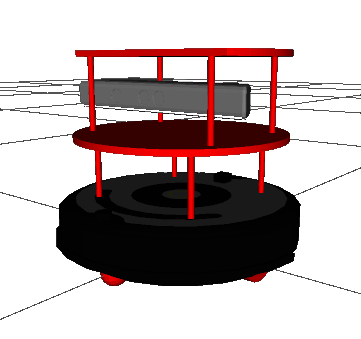
\includegraphics[scale=0.5]{./Figures/lubobot_urdf.png}
  \caption{Vista frontal del modelo URDF de Lubobot representado en RViz.}
  \label{fig:lubobotURDF}
\end{figure}

\begin{figure}[ht]
  \centering
  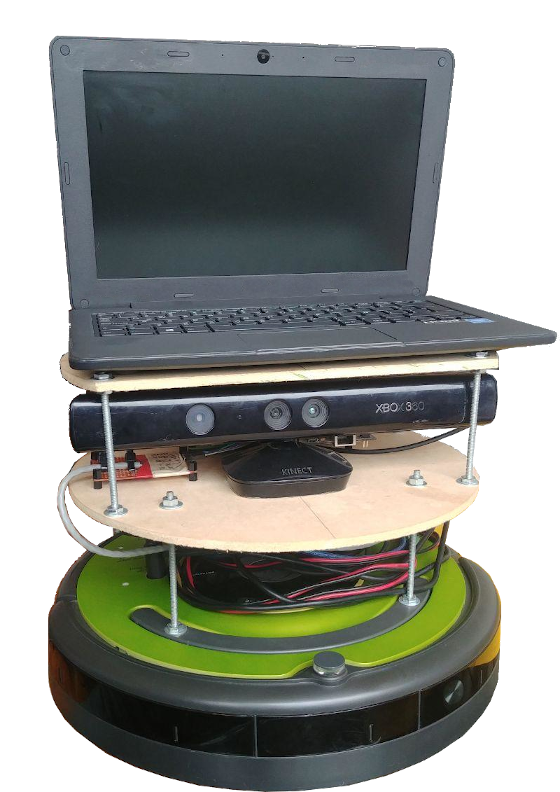
\includegraphics[scale=0.5]{./Figures/lubobot.png}
  \caption{Fotografía frontal del montaje del robot Lubobot.}
  \label{fig:lubobotReal}
\end{figure}

\newpage

Sobre la base móvil se montaron cuatro varillas roscadas de 5 mm de diámetro y 80 mm de largo, de las cuales las dos frontales fueron fijadas a la agarradera o  \textit{handler} del Roomba, mientras que las dos traseras se fijaron directamente al chasis. Dicha disposición fué calculada en base a las áreas del robot que el autor determinó como seguras para su modificación, es decir que no representaban ningún riesgo al correcto funcionamiento de la base móvil.

\subsection{Disposición de componentes}

Los diferentes componentes funcionales del robot fueron dispuestos en la configuración que se aprecia en la figura \ref{fig:lubobotComponentes}, a excepción de la \textit{laptop}, presente solo para fines de ejemplo ya que no forma parte del robot. Para la disposición propuesta se tuvieron en cuenta los siguientes criterios:

\begin{itemize}
  \item Mantener bajo el centro de gravedad del conjunto.
  \item Maximizar el espacio libre en el nivel superior para futuros \textit{upgrades}.
  \item Posicionar la IMU lo mas cerca posible del centro de rotación de la base y lo mas abajo posible.
  \item Posicionar el sensor Kinect a alrededor de 30 cm del suelo para incrementar su línea de visión.
  \item Mantener libre de obstrucciones el acceso al botón central del Roomba.
\end{itemize}

\begin{figure}[ht]
  \centering
  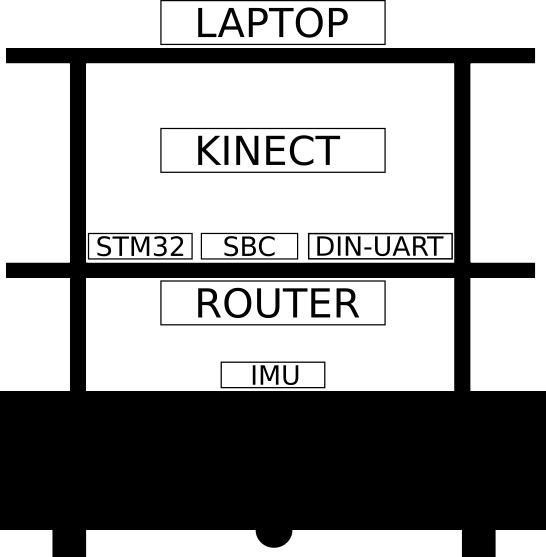
\includegraphics[scale=0.4]{./Figures/distribucion_componentes.png}
  \caption{Distribución de componentes del robot.}
  \label{fig:lubobotComponentes}
\end{figure}

\section{Diagrama en bloques de conexiones}

En la figura \ref{fig:lubobotComponentes} se muestra el diagrama de conexiones entre los distintos componentes electronicos del sistema y se indica además, el protocolo utilizado para cada interacción. Se decidió dotar al robot de un \textit{router} wifi a bordo de modo a facilitar su conexión a una computadora externa, destinada como estación de control para el envío de misiones.

\begin{figure}[ht]
  \centering
  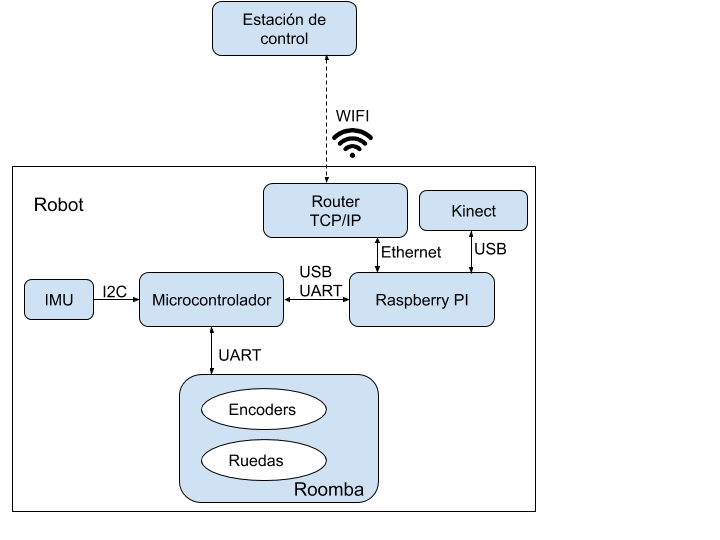
\includegraphics[scale=0.5]{./Figures/lubobot_conexiones.png}
  \caption{Diagrama de conexiones de los componentes constitutivos del robot.}
  \label{fig:lubobotComponentes}
\end{figure}

\newpage

\section{Implementación de firmware}

En esta sección se detallan las decisiones de diseño e implementación del firmware, encargado de la interconexión del robot Roomba y la Raspberry PI así como también de la lectura de sensores ajenos a la base móvil original como lo es la IMU.

\subsection{Distribución de tareas en FreeRTOS}

Debido a la necesidad de atender rutinas naturaleza tanto síncrona como asíncrona en el firmware, se decidió utilizar un RTOS para su implementación. Las tareas involucradas se describen a continuación, agrupadas en base a su responsabilidad dentro del sistema.

\subsection{Interfaz Roomba-microcontrolador}

Este conjunto de tareas cumplen la función de \textit{proxy} entre la base móvil Roomba y el resto del sistema. El microcontrolador se ocupa de la serialición y des-serialización de los paquetes intercambiados con el robot mediante el protocolo Open Interface, detallado en la sección \ref{sec:openInterface}. Las tareas responsables del manejo de esta función se describen en el apartado siguiente.

\begin{itemize}
  \item \textbf{Solicitud de lectura de sensores}: realiza la lectura de cada uno de los dos encoders disponibles de manera periódica cada 100 ms, actualizando las variables internas de estado en cada iteración con el valor actualizado.
  \item \textbf{Envío de comandos a actuadores}: realiza el despacho de comandos a los distintos actuadores disponibles en base a las órdenes recibidas desde ROS. Si bien esta tarea puede considerarse de carácter asíncrono, se implementó en la misma un mecanismo de \textit{watchdog} para evitar que un posible fallo en la comunicación con ROS ponga en peligro la integridad del usuario y del robot. Para esto, la tarea verifica cada 100 ms la existencia de un comando de velocidad nuevo. En su ausencia, envía una orden para detener el robot.
\end{itemize}

\subsection{Interfaz microcontrolador-ROS}

Esta interfaz involucró la migración de la biblioteca rosserial, mencionada en la sección \ref{sec:rosserial}, que hace posible entablar una comunicación serial asíncrona entre el microcontrolador y el una computadora corriendo ROS mediante su protocolo de mensajes estándar.

\begin{itemize}
  \item \textbf{Spin de ROS} esta tarea se encarga de llamar al método \file{spin} de la biblioteca rosserial manera periódica. Esta cumple la función de \textit{heartbeat} para la comunicación con la computadora, donde ambas partes se indican mutuamente si existen mensajes o servicios que transmitir.
  \item \textbf{Suscriptor de ROS} recibe los mensajes y solicitudes de servicios que fueron enviados desde ROS al microcontrolador y llama a las funciones de \textit{callback} requeridas para cada uno de ellos.
  \item \textbf{Publicador de ROS} despacha los mensajes y solicitudes de servicios que salen del microcontrolador.
\end{itemize}

\section{Implementación de software}

En esta sección se entra en detalle sobre la organización del código y archivos que acompañan al robot propuesto en este trabajo.

\subsection{Metapaquete Lubobot para ROS}

En esta sección se explica la estructura del meta-paquete Lubobot, que contiene las herramientas mínimas necesarias para comandar, modificar e inspeccionar el robot con ROS.

Como se describió en la sección \ref{sec:organizacionArchivos}, se considera una buena práctica el utilizar un metapaquete para contener varios paquetes que estan relacionados entre sí. Siguiendo estas recomendaciones, el software que acompaña al robot propuesto se organiza de la siguiente manera:

\begin{itemize}
  \item \textbf{lubobot\_description} incluye los archivos de descripción del robot en formato URDF y los archivos de visualización para RViz.
  \item \textbf{lubobot\_msgs} incluye los mensajes utilizados para intercambiar información entre el firmware y ros, a través de rosserial.
  \item \textbf{lubobot\_drivers} incluye el código de fuente para los nodos o programas que monitorean los sensores del robot, así como los que envían comandos a los actuadores.
\end{itemize}

\subsection{Nodo re-publicador de IMU ``lubo\_imu\_relay''}

Se encuentra suscripto a los mensajes del tipo \file{lubo\_imu}, compuesto por las lecturas crudas de orientación y aceleración angular provenientes del microcontrolador. El programa se encarga de procesarlos a medida que llegan, agregandoles información de tiempo y secuencia y luego los republica en el formato de mensaje estándar de ROS para unidades de medición inercial\protect\footnotemark.

Cabe preguntarse por qué de no evitar este nodo y publicar mensajes con el tipo estándar directamente desde el microcontrolador. Hay un par de motivos específicos que son válidos no solo para este mensaje en particular, sino también para la gran mayoría de los mensajes intercambiados con el microcontrolador:
\begin{itemize}
  \item los mensajes estandar de ROS poseen un \textit{footprint} en memoria poco adecuado para dispositivos con poca memoria RAM.
  \item el bus UART utilizado para la comunicación con el microcontrolador ofrece un ancho de banda ajustado que se satura rápidamente con mensajes del tipo estándar.
\end{itemize}

\footnotetext{Definición de mensaje estándar de ROS para Imu \url{http://docs.ros.org/kinetic/api/sensor_msgs/html/msg/Imu.html}}

\subsection{Nodo publicador de odometría ``lubo\_odom\_node''}

Está suscripto a los mensajes del tipo \file{lubo\_encoders} que provienen del microcontrolador. El mensaje se compone de las lecturas de los encoders izquierdo y derecho de la base Roomba. Cabe mencionar que las lecturas de ambos encoders deben tomarse en simultaneo para el correcto cálculo de la odometría, es por esto que el mensaje utilizado incluye ambas lecturas.

El microcontrolador publica los mensajes a una frecuencia por defecto de 20 hz, pero este y otros parámetros son también configurables desde la estación de control en \textit{runtime}. Esto se logra gracias al mecanismo de configuración \file{rosparam}, que ahorra la necesidad de recompilar el código cada vez que es necesario actualizar parámetros.

\subsection{Configuración del paquete ros\_localization}



\subsection{Configuración del paquete de navegación de ROS}

\section{Documentación en formato Wiki}

Se ofrece en conjunto con el repositorio Git\protect\footnotemark[2], una sección aparte dedicada exclusivamente a la documentación del robot. Para este fin se utilizó la funcionalidad de \textit{Wiki} ofrecida por la plataforma Github.

\footnotetext[2]{Repositorio principal del proyecto Lubobot \url{https://github.com/apojomovsky/lubobot}}


En la figura \ref{fig:wiki} se muestra la página principal de la \textit{Wiki} en su primera iteración, donde se realiza una breve presentación del proyecto, seguido de \textit{links} de interés con tutoriales y especificaciones técnicas.

\begin{figure}[ht]
  \centering
  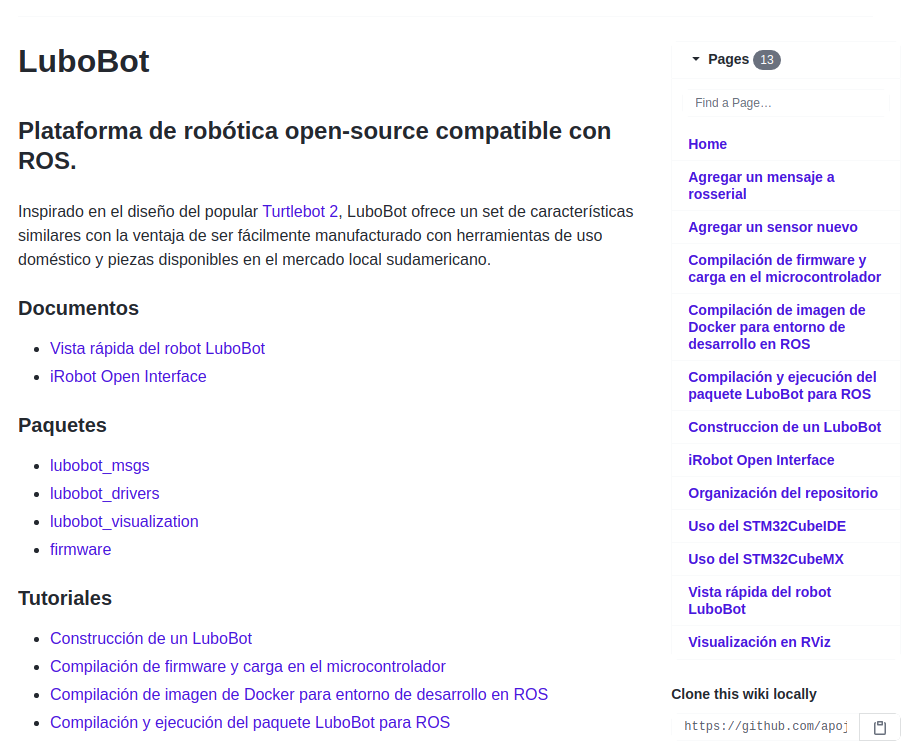
\includegraphics[scale=0.4]{./Figures/wiki.png}
  \caption{Página principal de la \textit{wiki} de LuboBot.\protect\footnotemark[3]}
  \label{fig:wiki}
\end{figure}

\footnotetext[3]{Wiki del proyecto Lubobot \url{https://github.com/apojomovsky/lubobot/wiki}}

Se decidió utilizar este formato de documentación en favor de incluir todo en el archivo \file{README.md} por una suma de motivos entre los que se destacan:

\begin{itemize}
  \item organización de archivos en un sub-repositorio proveído de manera automática por Github, con historial de cambios separado del repositorio principal.
  \item estructura de archivos múltiples organizados en forma de árbol, que no solo facilitan la búsqueda de información por parte del usuario sino que también facilita las tareas de mantenimiento.
  \item generación automática de índice en forma de \textit{sidebar} en el sitio que facilita la navegación entre las páginas que componen el sitio.
\end{itemize}
